%!TEX program = xelatex
\documentclass[10pt, compress, handout]{beamer}
\usepackage[titleprogressbar]{../../cls/beamerthemem}

\setbeamertemplate{caption}[numbered]
\setbeamertemplate{theorems}[numbered]
\newcounter{example}
\resetcounteronoverlays{example}
\newtheorem{crl}{Corollary}[theorem]
\newtheorem{eg}[example]{Example}
\newtheorem*{solution*}{Solution}

\usepackage{booktabs}
\usepackage[scale=2]{ccicons}
\usepackage{minted}

\usepackage{cleveref}
\crefname{example}{Example}{Examples}

\usepgfplotslibrary{dateplot}

\usemintedstyle{trac}

\usepackage{algorithm}
\usepackage[noend]{algpseudocode}
\resetcounteronoverlays{algorithm}

\usepackage{version}
% \excludeversion{proof}
% \excludeversion{solution*}

\usepackage{mathtools}
\usepackage{multicol}
\usepackage{qtree}

\usepackage{tikz}

\makeatletter
\def\old@comma{,}
\catcode`\,=13
\def,{%
    \ifmmode%
    \old@comma\discretionary{}{}{}%
    \else%
    \old@comma%
    \fi%
}
\makeatother

\title{CSCI 3190 Tutorial of Week 12}
\subtitle{Tree}
\author{LI Haocheng}
\institute{Department of Computer Science and Engineering}

\begin{document}

\maketitle

\begin{frame}[fragile]
\frametitle{Newark}
\onslide<1->\begin{columns}
    \begin{column}{.5\linewidth}
        \begin{eg}
            Find a shortest route in distance between Newark and
            Camden, and between Newark and Cape May, using
            these roads.
        \end{eg}
    \end{column}
    \begin{column}{.5\linewidth}
        \begin{figure}
            \centering
            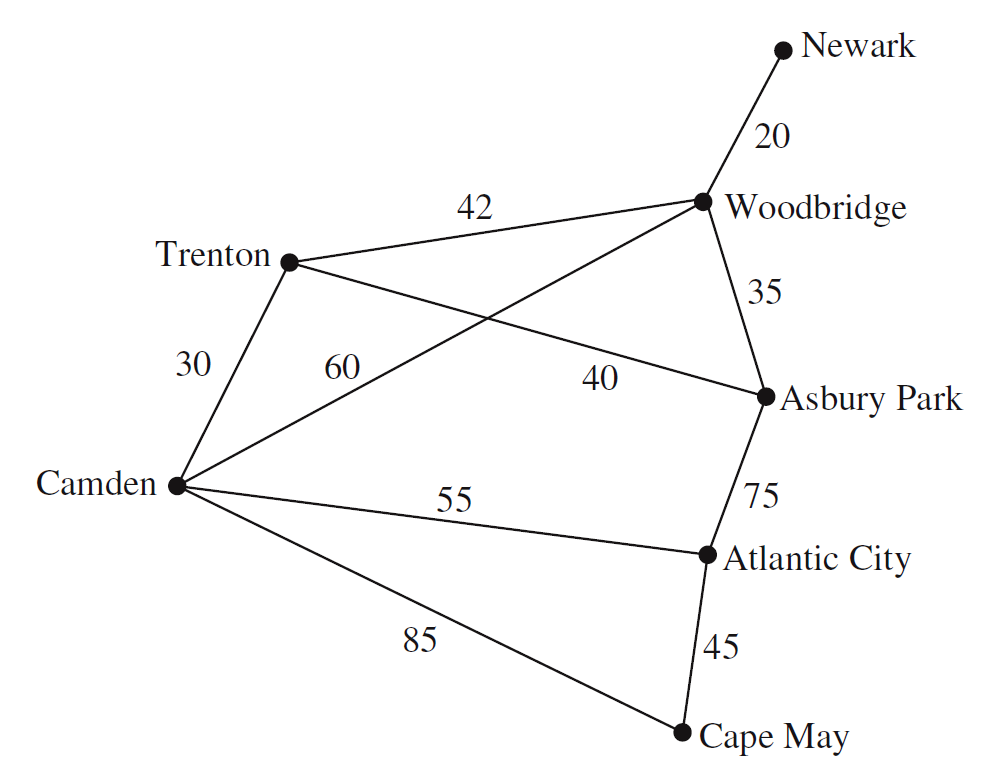
\includegraphics[width=\linewidth]{f-10-6-e-17-a}
        \end{figure}
    \end{column}
\end{columns}
\onslide<2>\begin{solution*}
    \begin{description}
        \item[Camden] 80
        \item[Cape May] 165
    \end{description}
\end{solution*}
\end{frame}

\plain{Questions?}

\end{document}
